\chapter{Pāli Root Finder}\label{chap:rootfinder}

This tool is newly added in \textsc{Pāli\,Platform\,3}. It lists all roots known by the Pāli traditions, collected in four books, namely \emph{Pāli Dhātupāṭha} (Dhāp), \emph{Kaccāyana-dhātumañjūsā} (Dhmjs), \emph{Saddanīti Dhātumālā} (Sadd-Dhā), and \emph{Dhātvatthasaṅgaha} (Dhātva).

The first book is used by Moggallāna school of Pāli grammar, the second by Kaccāyana school, the third by Saddanīti school. The last one is a recent collection composed by the Thera of Visuddhārāma in Mandalay, finished in 1889. Except the first book, all these works can be found in the collection of Traditional Pāli Grammar Books.\footnote{In printed form, \emph{the Pāli Dhātupāṭha and the Dhātumañjūsā} were edited by Dines Andersen and Helmer Smith (1921), \url{archive.org/details/palidhatupathadh00andeuoft}. Saddanīti Dhātumālā was edited by Helmer Smith (1929), \url{archive.org/details/SaddanitiAggavamsasPaliGrammar02}. As far as I know, there is no Western edition of Dhātvatthasaṅgaha. I saw one Thai edition, and there are possibly some Myanmar editions.}

When you first open the Root Finder window, you will see the grand table of 5,547 roots, variants included (see Figure \ref{fig:root-finder}). Each row of the table shows the reference to the book, the root's name, its Pāli definition\footnote{For English definition, please see in Roots window (Chapter \ref{chap:roots}). Even if it is not exhaustive there, it covers most of them.}, and the root's group. When {\faSix \symbol{"F0AE}} toggle button is clicked, the selectors of books and root groups will be shown or hidden. 

\begin{figure}[!hbt]
\centering
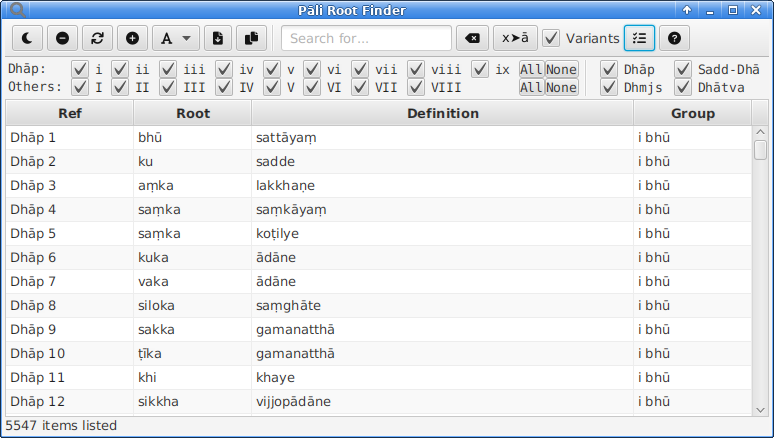
\includegraphics[width=0.9\linewidth]{images/root-finder.png}\\
\caption{Window of Pāli Root Finder}
\label{fig:root-finder}
\end{figure}

Concerning root groups, there are some disagreements we should know. In Dhātupāṭha, the groups are divided into nine, in Dhātumañjūsā seven (according to Andersen and Smith's book), and in Dhātumālā and Dhātvatthasaṅgaha eight. To make our life a little easier, I changed groups in Dhātumañjūsā to eight, conforming to the most-used Kaccāyana-Saddanīti scheme.\footnote{In the book by Andersen and Smith, Dhātumañjūsā does not have group VI (gaha), but VI (tanu) and VII (cura). The last two are changed to VII (tanu) and VIII (cura). The word \pali{gaha} itself belongs to group V (kī) in this book.} And to differentiate the two schemes, I use lowercase Roman numbers for the 9-group and uppercases for the 8-group. The comparison of two schemes of root groups is shown in Table \ref{tab:root-groups}.

\begin{table}[!hbt]
\centering
\caption{Root groups}
\label{tab:root-groups}
\bigskip
\begin{tabular}{ll} \toprule
\bfseries 9-group scheme & \bfseries 8-group scheme \\ \midrule
i (bhū) & I (bhū) \\
ii (rudha) & II (rudha) \\
iii (diva) & III (diva) \\
iv (tuda) & IV (su) \\
v (ji) & V (kī) \\
vi (kī) & VI (gaha) \\
vii (su) & VII (tanu) \\
viii (tana) & VIII (cura)  \\
ix (cura) &  \\
\bottomrule
\end{tabular}
\end{table}

Let us talk about variants a bit. Because I use texts from various sources, there are discrepancies among them. So, I include all of them, and mark roots from secondary source as \emph{variant}. Sources of data used in this tool are listed below, and summarized in Table \ref{tab:root-sources}.

\begin{compactitem}
\item Dhātupāṭha has only one source (Andersen and Smith's book), so there are no variants in this book.
\item The main source of Dhātumañjūsā is the Chaṭṭha Saṅgā\-yana collection. The text is edited using a Thai edition (Wat Chakdaeng, 2013). So, this book has two sources of variants: \emph{sy} (Syāma = Thai), and \emph{as} (Andersen and Smith).
\item The main source of Dhātumālā is the Chaṭṭha Saṅgāyana collection. This is checked against a Thai (Bhūmibalo edition, 2016) and Smith's edition. So, it has two sources of variants: \emph{sy} and \emph{sm} (Smith).
\item The digital form of Dhātvatthasaṅgaha is taken from \emph{Palipage}\footnote{\url{sites.google.com/view/palipage}}. This is checked against a Thai edition of Dhā\-tvatthasaṅgahapāṭhanissaya (MCU Press, 1992). So, it has one source of variants as \emph{sy}.
\end{compactitem}

\begin{table}[!hbt]
\centering
\caption{Sources of root data}
\label{tab:root-sources}
\bigskip
\begin{tabular}{lll} \toprule
\bfseries Books & \bfseries Main & \bfseries Variants \\ \midrule
Dhātupāṭha & as & -- \\
Dhātumañjūsā & CST & sy, as \\
Dhātumālā & CST & sy, sm \\
Dhātvatthasaṅgaha & Palipage & sy \\
\bottomrule
\end{tabular}
\end{table}

The use of this tool is simple and obvious. So, it needs no further explanation. The root finder has its parallel web version at \url{bhaddacak.github.io/paliroot}. This has some explanations not included here, and it is somewhat handier to use.
